\title{CSCI 274 - Introduction to Linux \\Course Syllabus \\Sections A, B, and C}
\date{\vspace{-25pt} Spring 2018}
\documentclass[12pt]{article}
\usepackage{hyperref}
\usepackage{enumitem}
\usepackage{graphicx}
\begin{document}
  \maketitle
\begin{description}
  \item[Instructor] Sam Schilling
  \item[Email] \texttt{sschilli@mines.edu}
  \item[Lecture Times]
  
  \item Section A - M 2:00  PM MST
  \item Section B - W 1:00  PM MST
  \item Section C - F 12:00 PM MST
  
  \item[Classrooms]
  
  \item Section A - BB 253
  \item Section B - CT B60
  \item Section C - BB 316A
  
  \item[Office Hours] BB W378 
  
  \item W 2:00-3:00 PM MST
  \item F 1:00-2:00 PM MST
  \item[TA] Qin Yang, \texttt{qinyang@mymail.mines.edu}
  \item[TA Office Hours] TBD
  \item[Course Webpage] \href{https://sschilli.github.io}{https://sschilli.github.io}
  % \item[Course Piazza] \href{https://piazza.com/class/izqhwpn1h892h1?cid=6}{https://piazza.com/class/izqhwpn1h892h1?cid=6}
\end{description}
% ==================================================
\section{Course Description}
Introduction to the Linux Operating System will teach students how to become proficient with using a Linux operating system from the command
line.

\paragraph{Topics} remote login (ssh), file system navigation, file manipulation commands, editors, i/o redirection, searching, search and replace,
processes, pipelines, file system interrogation commands, authentication, permissions, compression, privacy, and bash scripting

\paragraph{Prerequisites: CSCI 261. 1 hour lecture; 1 semester hour.}
% ==================================================
\section{Learning Goals}
The objective of this course are to introduce students to the GNU/Linux operating system:

\begin{enumerate}
  \item The command-line interface to essential utilities
  \item Editing text files
  \item Shell scripting environment (bash)
  \item Utilizing other system utilities for efficient programming and administration tasks
  \item Basic authentication, integrity, and privacy commands 
\end{enumerate}

Upon completion of this course, you should know:
\begin{itemize}
  \item How to navigate the filesystem, invoke applications with i/o redirection, and connect applications with pipelines.
  \item Efficiently use a text editor for many various tasks, including the authoring of shell scripts.
  \item How to connect to remote machines through TCP/IP based networks.
  \item Author basic Bourne shell scripts (bash). 
\end{itemize}
% ==================================================
\section{Computer Facilities and Assistance}
You need an ADIT account to use the lab machines in the Computer Commons, library, and CTLM, which most students create during EPICS. If you do not
have an ADIT account, you need to know your eKey (personal identification code used to create your webmail account) and visit
\href{http://newuser.mines.edu/adit} prior to the first lab. If you do not know your eKey, contact the Computer Commons Help Desk in room 156A of CTLM.
% ==================================================
\section{Grading Policy}
\begin{description}
  \item{30\%} Assignments
  \item{25\%} Midterm Exam
  \item{45\%} Final Exam
\end{description}

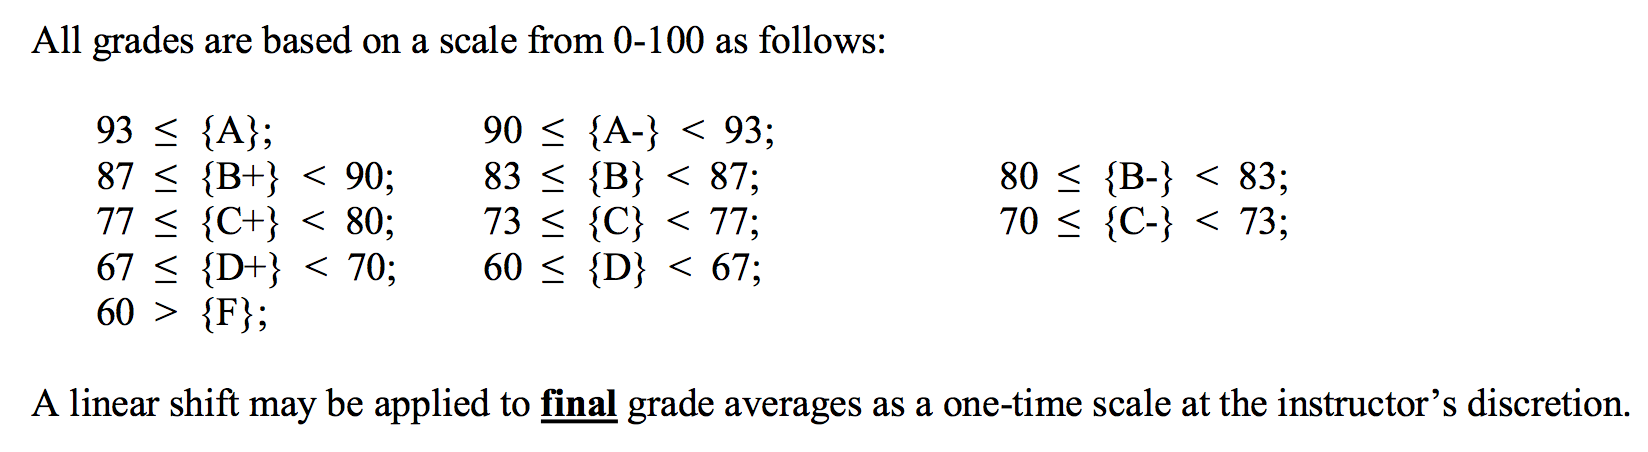
\includegraphics[width=\linewidth]{scale}
  
\paragraph{Late Policy}
Late Policy: 10\% off for first 24 hours, 15\% off for second 24 hours, 40\% of for the third 24 hours (3 days late). Assignments posted 4 days or more
after the due date are not graded. Weekends count as late days, all work must be turned in by midnight on the day of the final exam.

\paragraph{Pass the Exams to Pass the Course}
Students must have a midterm quiz and final exam weighted average $\geq$ 60\% to pass. This weighting is based on the point value of the two assessments,
not the course grade weights in the table above!
% ==================================================
% \section{Piazza}
% This term we will be using Piazza for class discussion. The system is highly catered to getting you help fast and efficiently from classmates, the TA,
% and myself. Rather than emailing questions to the teaching staff, I encourage you to post your questions on Piazza. If you have any problems or
% feedback for the developers, email \texttt{team@piazza.com}.

\section{Assignments}
Scripting and written assignments may we worth different numbers of points, but their percentile grades are all weighted the same when calculating
the ``Assignment'' portion of your course grade.

Written assignments include Google Forms distributed periodically throughout the course.

\subsection{Reading Assignments}
Unix and Unix-like operating systems (Linux, FreeBSD, \dots) have a long history of providing both development tools (compilers, editors, software
management tools) as well as complete documentation for free and online. In this sense, online does not mean the Internet; rather it means
documentation in an electronic form installed along side the system applications.

As such, we won't need a textbook for this course.

Reading assignments will be collectively graded as a writing assignment at the end of the course based on the quality of the \texttt{CHEATSHEET.LNX} file created. As
discussed at the beginning of the course, this file is a running set of notes for your reference and you should format/add to it as you see fit.

\subsection{Scripting Assignments}
For Scripting Assignments, any malicious commands will be considered a form of academic misconduct (e.g., don't try to exploit the fact that I might
blindly run your scripts sometimes).

No partial credit will be given to scripts that do not have sufficient comments (remember: \texttt{\#} is the comment character in \texttt{bash}).
% ==================================================
\section{Exams}
\paragraph{``No Show'' Policy}
Failure to sit for a scheduled exam (without a really good explanation) incurs the same ``late penalty'' as for late assignments in the course. The
``lateness'' is measured between the scheduled exam time and when your instructor or course coordinator is informed of your absence.
Beyond this (again, without an incredibly good explanation) a zero will very likely be recorded for the exam grade.

Students are not guaranteed the opportunity to take a make-up exam; leniency in these matters is at the discretion of the course instructor(s).
% ==================================================
\section{Collaboration Policy}
The following policy exists for all CS courses in the CS department. This policy is a minimum standard; your instructor may decide to augment this
policy.

\begin{enumerate}
  \item If the project is an individual effort project, you are not allowed to give code you have developed to another student or use code provided by another
    student. If the project is a group project, you are only allowed to share code with your group members.
  \item You are encouraged to discuss programming projects with other students in the class, as long as the following rules are followed:
    \begin{enumerate}
      \item You view another student's code only for the purpose of offering/receiving debugging assistance. Students can only give advice on what problems to
      \item look for; they cannot debug your code for you. All changes to your code must be made by you.
      \item Your discussion is subject to the empty hands policy, which means you leave the discussion without any record [electronic, mechanical or otherwise] of
        the discussion.
    \end{enumerate}
  \item Any material from any outside source such as books, projects, and in particular, from the Web, should be properly referenced and should only be used
    if specifically allowed for the assignment.
\end{enumerate}

\section{Disability Services}
Students with disabilities should contact the Disability Services to become aware of their rights and responsibilities. \\
\href{http://disabilities.mines.edu/}{http://disabilities.mines.edu/}
\section{Military and Veterans Services}
Military students and veterans should contact the Veterans Services to become aware of their benefits and responsibilities. \\
\href{http://inside.mines.edu/Veterans-Services}{http://inside.mines.edu/Veterans-Services}
\end{document}

